\section{Introduzione}
Prima di entrare nel dettaglio della nostra trattazione definiamo che cos'è un \emph{Linguaggio Formale.} Innanzitutto dobbiamo distinguere tra un \emph{linguaggio natura} ed uno \emph{artificiale}, un linguaggio naturale è quello che utiliziamo tutti i giorni e che si basa sul significato delle parole e soprattutto non possiede una struttura formale. Un linguaggio artificiale, invece, è quello utilizzato per la comunicazione tra macchine, è di tipo no verbale ma soprattutto è formale.\\
Un linguaggio si definisce \textbf{formale} se la sua \emph{sintassi} (ovvero la sua struttura) e la sua \emph{semantica} (ovvero il suo significato) sono definiti da precisi algoritmi. Questo permette di definire delle \emph{procedure} precise per determinare la correttezza di una frase che appartiene ad un linguaggio e il suo significato. 
In un contesto più ristretto un \textbf{linguaggio formale} è un \emph{oggetto matematico} costruito su di un \emph{alfabeto} tramite regole assiomatiche chiamate \emph{grammatiche} o tramite strumenti matematici chiamati \emph{automi}.\\
\subsection{Introduzione alla teoria dei linguaggi formali}
Vediamo ora alcune definizioni che ci saranno utili durante il corso:
\begin{description}
	\item[Alfabeto:] insieme \emph{finito} di elementi
	$$\Sigma = \{a_1, a_2, a_3, \dots, a_k\}$$
	\item[Cardinalità di un alfabeto:]  è il numero di elementi che lo compongono
	$$ |\Sigma| = k $$
	\item[Stringa:] insieme ordinato di elementi dell'alfabeto che possono essere anche ripetuti.
	$$\Sigma = \{a,b,c\}$$
	$$Stringe: \ abc \vee aab \vee ac \vee bbb$$
	\item[Linguaggio:] insieme finito o infinito di stringhe di un alfabeto
	$$L_1 = \{ab,ac,abc\}$$
	$$L_2 = \{bc,bbc,\dots\}$$
	La struttura insiemistica del linguaggio formale ha due livelli di profondità:
	\begin{itemize}
		\item Insieme non ordinato di elementi non atomici (\emph{stringhe}) che sono
		\item sequenze ordinate di elementi atomici (\emph{elementi o terminali}).
	\end{itemize}
	\item[Cardinalità di un linguaggio:] può essere finita o infinita.
	$$|L_1| = |\{ab,ac,abc\}| = 3$$
	\item[Lunghezza di una stringa:] indica il numero dei suoi elementi
	$$|abb| = 3 \quad |abbc| = 4$$
	\item[Uguaglianza tra stringhe:] due stringhe si definiscono uguali se e solo se hanno la stessa lunghezza, ed i suoi elementi coincidono ordinatamente da sinistra a destra.
	$$x = a_1a_2\dots a_h \quad y = b_1b_2\dots b_k$$
	$$x = y \iff h = k \wedge a_i = b_i \ \forall i = 1\to h $$
\end{description}
\subsubsection{Operazioni con le stringhe}
La \emph{concatenazione} è l'operazione fondamentale con le stringhe, si tratta di fare il prodotto tra esse. Questa operazione è un operazione di base e non fa altro che disporre in fila le due stringhe.
$$x = a_1a_2\dots a_h \quad y = b_1b_2\dots b_k$$
$$x\cdot y = a_1a_2\dots a_hb_1b_2\dots b_k = xy$$
Questo tipo di operazione gode della proprietà associativa e va ad influire sulla lunghezza della stringa come vediamo dalla \ref{eq:conass} e dalla \ref{eq:conlen}.
\begin{equation}\label{eq:conass}
	(xy)z = x(yz)
\end{equation}
\begin{equation}\label{eq:conlen}
	|xyz| = |x| + |y| + |z|
\end{equation}
La concatenazione ci permette di introdurre un altro concetto relativo alle stringhe, ovvero quello della \emph{stringa vuota} o \emph{nulla} indicata con $ \varepsilon $ questa stringa è l'elemento neutro rispetto all'operazione di concatenazione, infatti, concatenando $ \varepsilon $ a destra o a sinistra di una stringa la stringa non cambia.
$$\varepsilon x = x\varepsilon = x$$
Tuttavia bisogna prestare attenzione a non confondere la stringa nulla con l'insieme vuoto $Phi$.\\
Una volta capita l'operazione di concatenazione si possono individuare in una stringa delle \emph{sotto-stringhe}, ovvero stringhe più piccole concatenate tra loro per formare una stringa più grande.
Ad esempio data una stringa $x$ essa può essere vista come un insieme di sotto-stringhe concatenate
$$x = uyv$$
Dove:
\begin{itemize}
	\item \emph{y} è detta sotto-stringa.
	\item \emph{u} è chiamato prefisso.
	\item \emph{v} è chiamato suffisso.
\end{itemize}
Un esempio di suffissi, prefissi e sotto-stringhe è mostrato in \figurename\,\ref{fig:sufpref}.
\begin{figure}
	\centering
	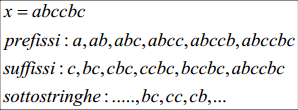
\includegraphics[width=0.5\linewidth]{img/substr.png}
	\caption{Esempio di sottostringhe con prefissi e suffissi}\label{fig:sufpref}
\end{figure}

Si definiscono \emph{sotto-stringhe proprie} tutte quelle stringhe che hanno $u\neq \varepsilon$ e $v \neq \varepsilon$